\chapter{\label{chap:entwurf}Konzeption}
% ### Design ###
\section{Das Design}
Hohe Kontraste wegen Wetter.\\
einfache UI .\\
Minimalistisch sodass ein Blick genügt und man nicht abgelenkt wird.\\
Angezeigt wird: Geschwindigkeit schneller oder langsamer, 
Restrotanzeige, grüne Welle.
\begin{figure}[H]
        \centering
           \begin{subfigure}[t]{0.23\textwidth}
                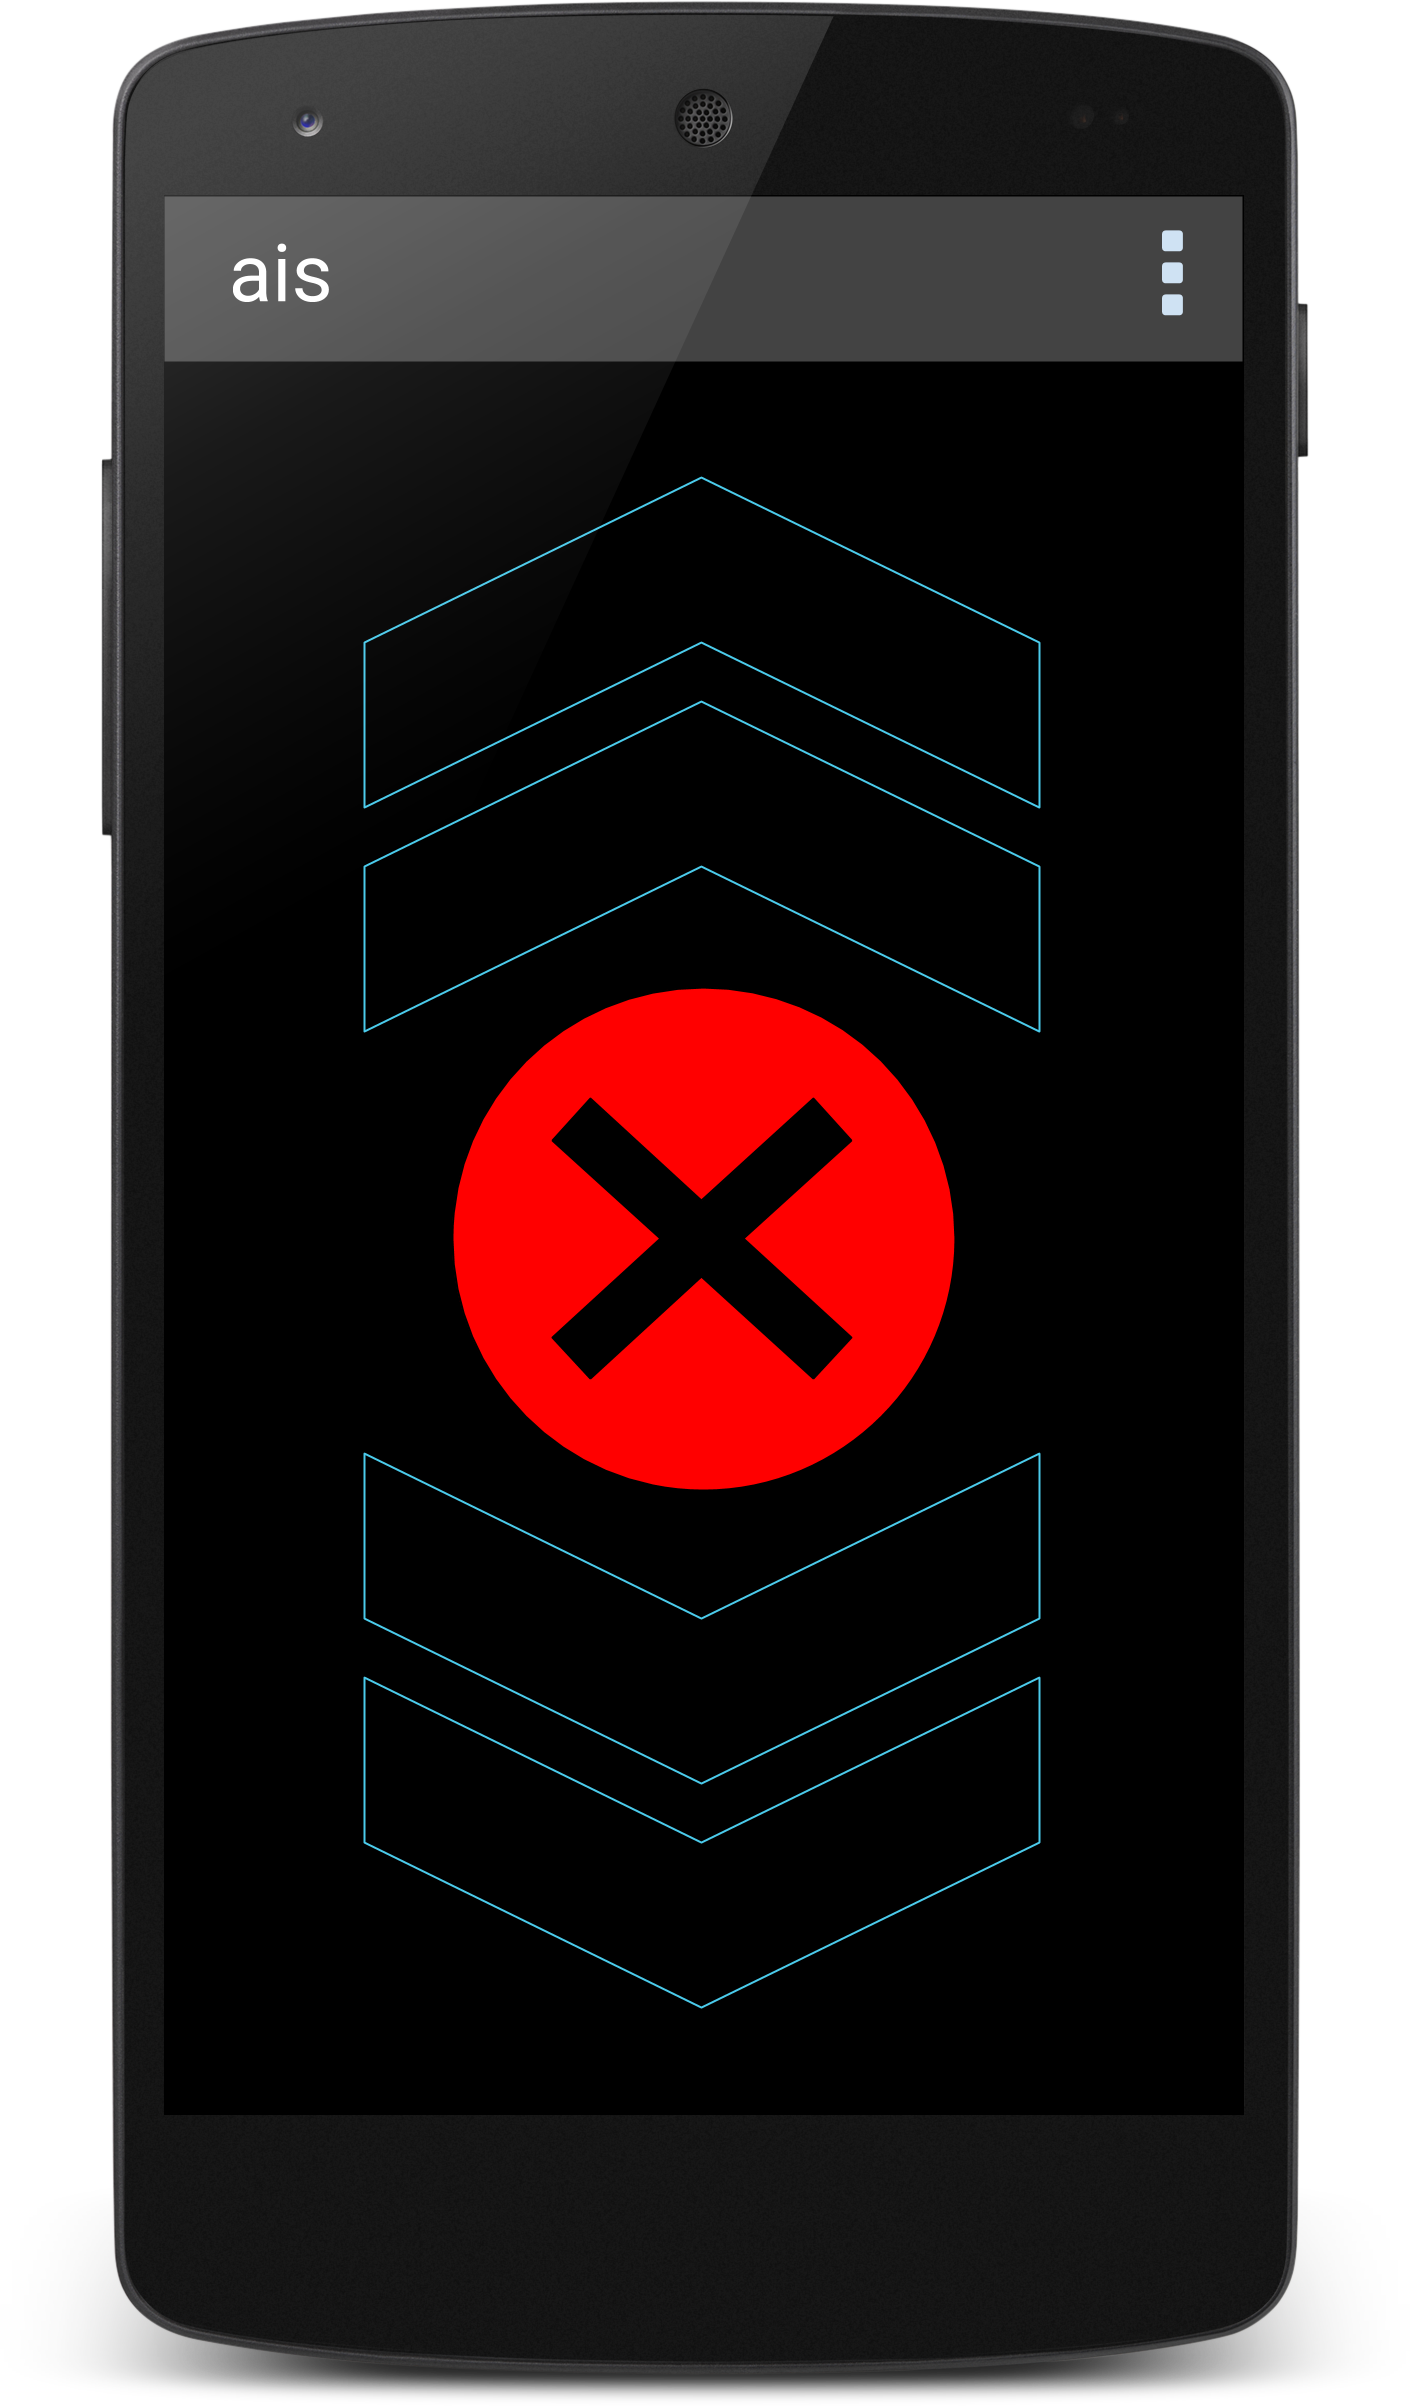
\includegraphics[width=\textwidth]{stop}
                \caption[Systemzustand d]{keine Weiterfahrt möglich}
                \label{fig:stop}
        \end{subfigure}
           ~ 
              \begin{subfigure}[t]{0.23\textwidth}
                
\includegraphics[width=\textwidth]{yeah}
                \caption[Systemzustand c]{Kein Aktionsbedarf}
                \label{fig:yeah}
        \end{subfigure}
           ~
        \begin{subfigure}[t]{0.23\textwidth}
                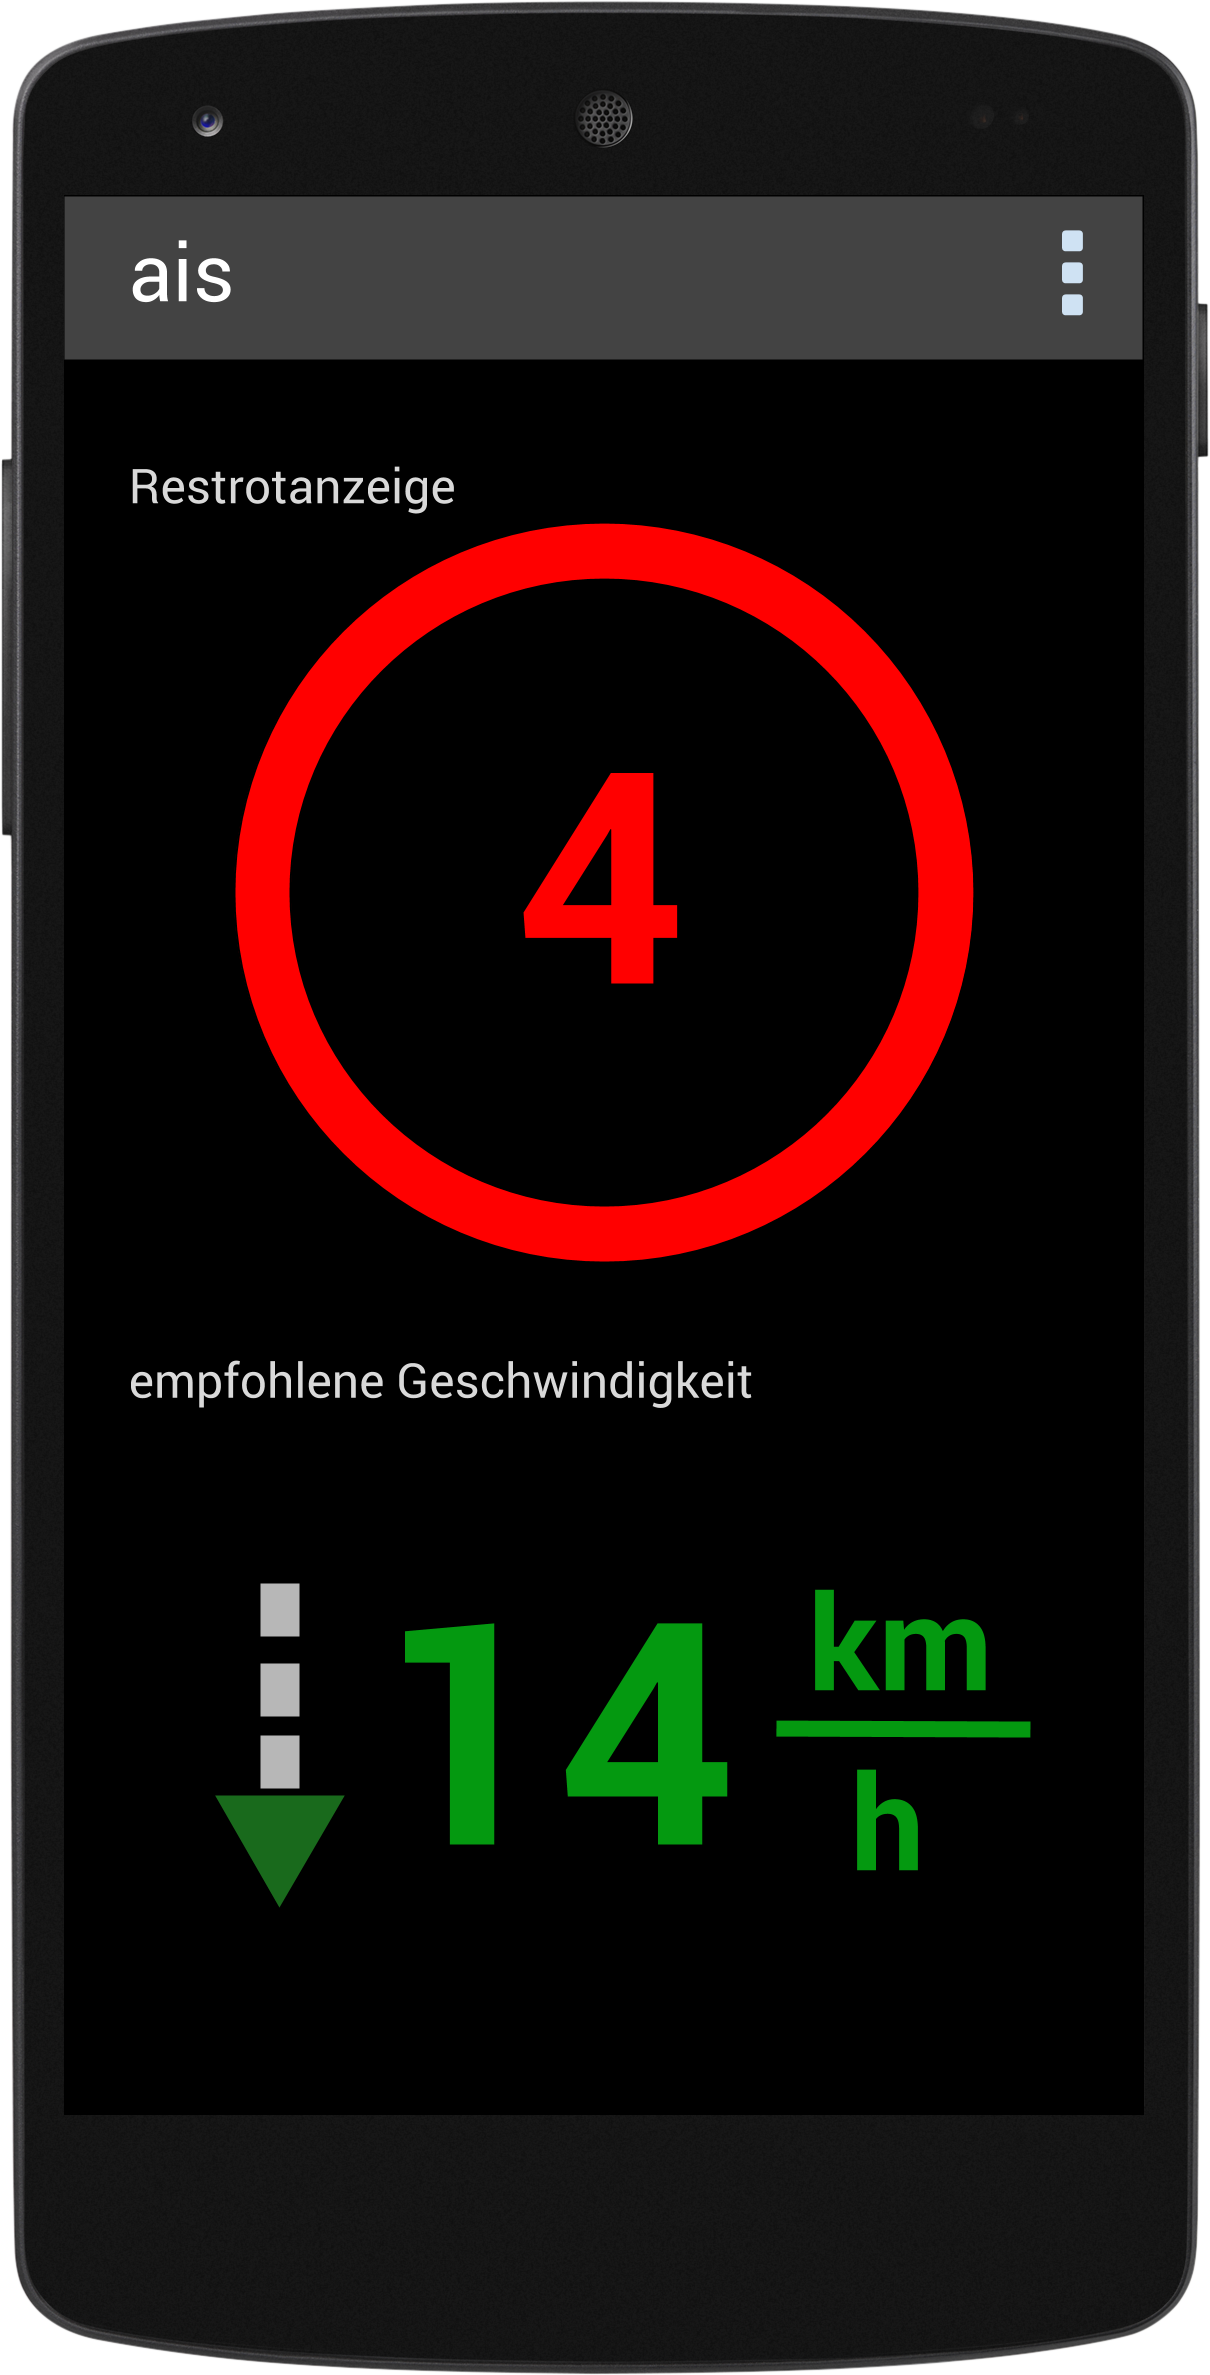
\includegraphics[width=\textwidth]{langsamer}
                \caption[Systemzustand a]{Weiterfahrt durch Verlangsamung  möglich}
                \label{fig:langsamer}
        \end{subfigure}
        ~
        \begin{subfigure}[t]{0.23\textwidth}
                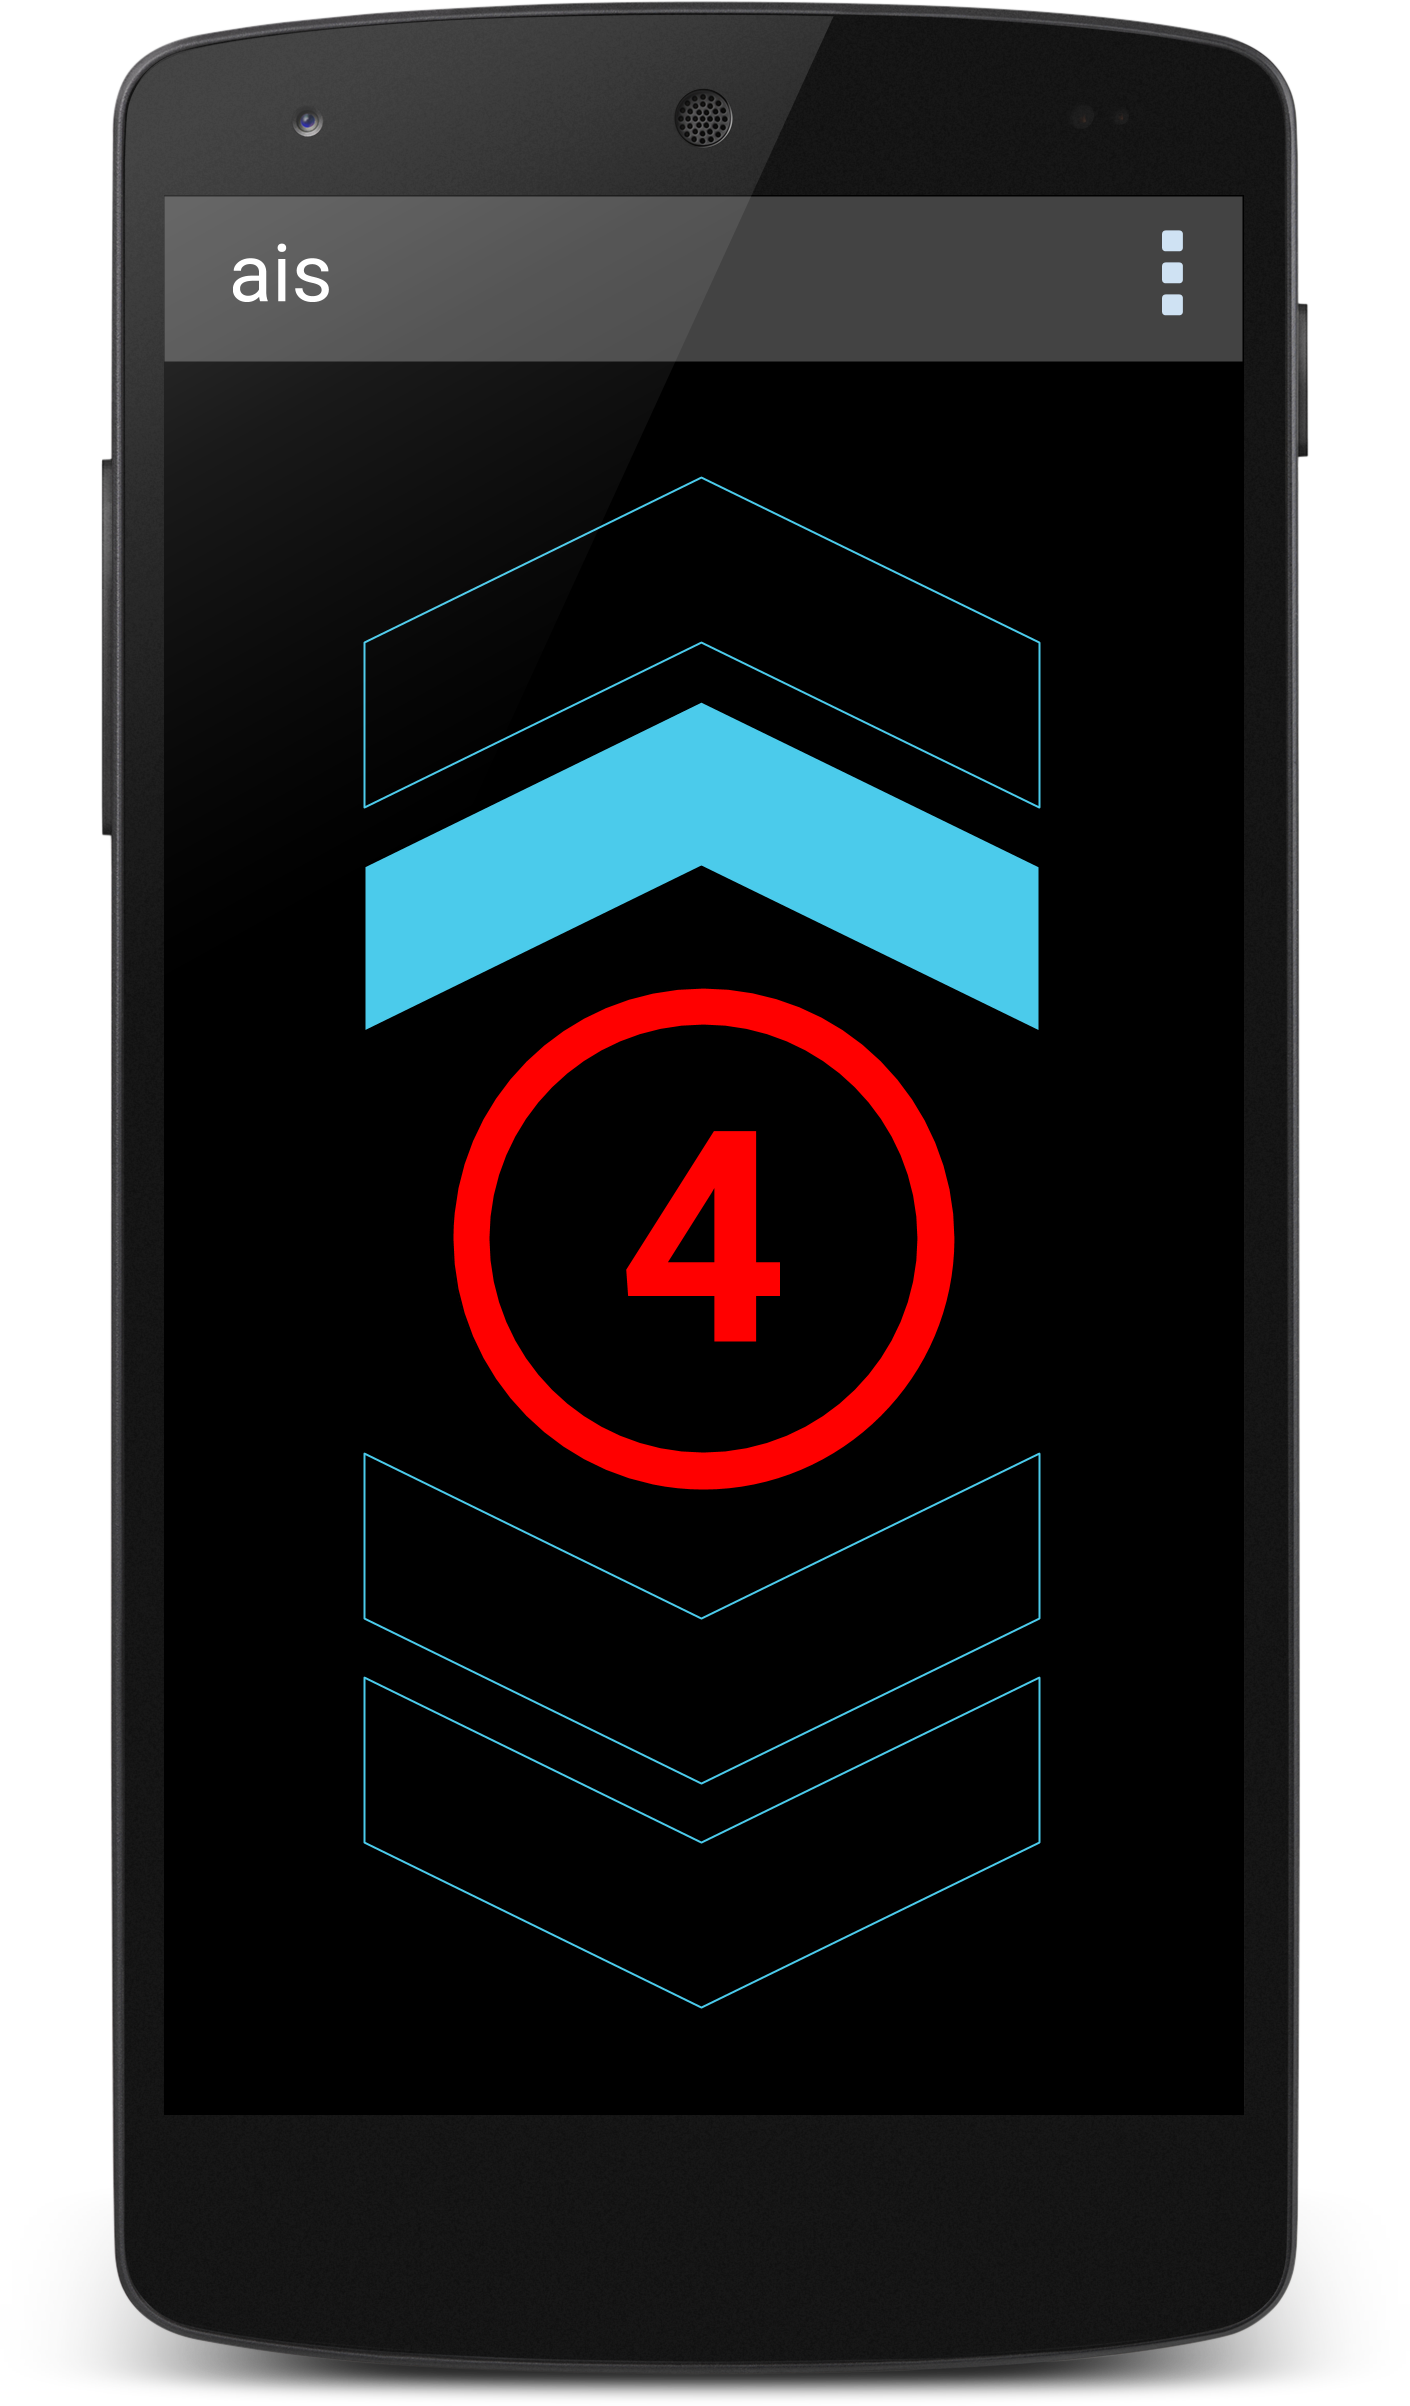
\includegraphics[width=\textwidth]{schneller}
                \caption[Systemzustand b]{Weiterfahrt durch Beschleunigung möglich}
                \label{fig:schneller}
        \end{subfigure}     
        \caption[Systemzustände im Ampelbereich]{Umsetzung des Designs anhand der Systemzustände}
        \label{fig:mockup}
\end{figure} 
\subsection{Anzeigeelemente}
\subsubsection{Geschwindigkeit}
\subsubsection{Ampeln}
\subsubsection{Informationen}
% ### Achitektur ###
\section{Architektur}
Klassenstruktur..
\subsection{Navigation}
\section{Ampeldatenanfrage und Auswertung}
\section{Theorie}
Um die korrekte Umsetzung des Prototyps zu ermöglichen, müssen zunächst einmal prinzipielle
Theorien und Hintergründe diesen betreffend betrachtet werden.
grundlegendes Wissen über geographische Koordinaten sowie mathematische Voraussetzungen im Umgang mit diesen, müssen zur Ideenverwirklichung berücksichtigt werden.
\subsection{Die Berechnung der Entferung}
\subsection{Die Berechnung der Ankunft in Abhängigkeit der Geschwindigkeit}
\subsection{Die Anzeige der Restrotanzeige}
